Section~\ref{sec.exp.setup2} gives details about our experimental setup for multi-fault programs. Section~\ref{sec.exp.subject2} introduces the subject programs used in our study. Sections~\ref{sec.exp.resultsA2}~\&~\ref{sec.exp.resultsB2} show the results.

\subsubsection{Experimental Setup}\label{sec.exp.setup2}

The overall experimental setup for the multi-fault setting is similar to the single-fault setting. However, we need to modify the diagnostic cost as now there are multiple faults. The diagnostic cost is defined as follows:

\begin{equation}\label{equation.avgcost}
	cost = \dfrac{\left|  \left\{ j \left| \right.
           f_{T_{\mathcal{S}}}(d_j) \geq \min_{\substack{d_* \in D*}} f_{T_{\mathcal{S}}}(d_*) \right\} \right|}
           {\left|  \mathcal{D} \right|}
\end{equation}

\noindent where $\mathcal{D}$ consists of all program elements appearing in the program.
We calculate the average cost as the percentage of elements that developers have
to examine until locating all root causes ($D_*$). Since multiple
program elements can be assigned with the same ambiguity score, the numerator
is considered as the number of program elements $d_j$ that have bigger or the
same ambiguity score to a root cause $d_*$ in $D_*$ with the
lowest
ambiguousness
score. In this setting, we consider the worst-case scenario where developers need
to find all root causes by inspecting all elements that have a score no lower than the score of any root cause.

%In our experiment, every test case prioritization technique starts from an arbitrary labeled failed trace because developers start debugging only when test cases fail.

%We compare the effectiveness of different prioritization methods based on the diagnostic cost when the same number of test cases are selected.

%The diagnostic cost is defined as follows:
%\begin{equation}\label{equation.avgcost}
%	cost = \dfrac{\left|  \left\{ j \left| \right. f_{T_{\mathcal{S}}}(d_j) \geq f_{T_{\mathcal{S}}}(d_*) \right\}  \right|}{\left|  \mathcal{D} \right|}
%\end{equation}
%where $\mathcal{D}$ consists of all program elements appearing in the program.
%We calculate the average cost as the percentage of elements that developers have
%to examine until locating the root cause($d_*$) of failure. Since multiple
%program elements can be assigned with the same suspicious score, the numerator
%is considered as the number of program elements $d_j$ that have bigger or the
%same suspicious score to $d_*$.
%
%In this paper, we use \textsc{Raptor} as the bootstrapping technique ($\mathcal{P}$ in Figure \ref{algo:DMS}). During the bootstrapping process, $w$ is set to 10 to facilitate trend analysis.
%
%Following~\cite{JiangCT11}, for each faulty version, we repeat each prioritization technique 20 times to obtain its average cost. For each time, a randomly chosen failed trace is used as the starting point to alleviate the sensitivity of the technique to the choice of starting traces. On the other hand, to fairly compare our approach with other prioritization methods, the {\em same randomly} chosen failed traces are used as the starting traces for all methods.

\subsubsection{Subject Programs}\label{sec.exp.subject2}

Each multi-fault program version used in our study contains more than one bug where each bug involves only one line (or one simple statement if the statement is broken into more than one line) in the program and different bugs affect different lines. This consideration is aligned with previous studies \citep[e.g.][]{zhang2013bridging,Abreu:2009.jss}. We use a dataset containing 173 multi-fault versions of 8 C programs as shown in Table~\ref{tab:multibug}. Different versions may contain the same fault, and there are 157 distinct faults in total. The dataset was previously used by \cite{lucia2013} to evaluate 40 different association measures.

%As print_token and schedule2 datasets only have four and seven bugs that involve one line, we randomly insert two bugs for every version, whereas for other datasets, we randomly insert five bugs for every multiple-bug version. Also, we ensure that each bug has been inserted at least in one of the versions. We generate multiple-bug versions for each dataset as many as the number of single-bug versions in the dataset. For example, there are 38 single-bug versions for Space, so we randomly generate 38 multiple-bug versions for Space, each of which contains five bugs. For each print_tokens and schedule2 dataset, we generate 10 multiple-bug versions. Thus, we have 20 multiple-bug versions that contain two bugs (minimum number of multiple bugs) and 153 versions that contain five bugs.

\begin{table}[!htbp]
	%\vspace{-8pt}
	\centering
	\caption{multi-fault Subject Programs}\label{tab:multibug}
	\renewcommand{\arraystretch}{1.5}
	%\small
    \begin{tabular}{|l|c|c|c|} \hline
        Program & \# Bugs Per Version &\# Tests& \# Versions\\ \hline\hline
		tcas & 5 &1,608& 41\\ \hline
        schedule2 & 2& 2,710 & 10\\ \hline
        schedule & 5&2,650 & 9\\ \hline
        replace & 5&5,542 & 32\\ \hline
		tot\_info & 5 &1,052 & 23\\ \hline
        print\_tokens2 & 5 &4,115& 10\\ \hline
        print\_tokens & 2&4,130 & 10\\ \hline
        space & 5&1,343 & 38\\ \hline
	\end{tabular}
	\label{dataset}
\end{table}


%We use five real {\em C} programs and seven Siemens test programs from the {\em Software-artifact Infrastructure Repository}~(SIR)~\cite{doESE05}. We refer to the five real programs (\texttt{sed}, \texttt{flex}, \texttt{grep}, \texttt{gzip}, and \texttt{space}) as \textsc{Unix} programs. Table \ref{dataset} shows the descriptive statistics of each subject, including the number of faults, available test cases and code size. Following \cite{JHS02,Abreu:2009.jss}, we exclude faults not directly observable by the profiling tool\footnote{http://gcc.gnu.org/onlinedocs/gcc/Gcov.html} (e.g., some faults lead to a crash before \texttt{gcov} dumps profiling information and some faults do not cause any test case to fail), and in total we study 254 faults.


\subsubsection{Experimental Results: Reducing Number of Test Cases}\label{sec.exp.resultsA2}
%In this subsection, we conduct several controlled experiments to show the effectiveness of \textsc{Dms}.

%\vspace{-4pt}
%\subsubsubsection{Effectiveness on Reducing The Number of Test Cases Needed for a Target Cost}

We investigate the effectiveness of \textsc{DMS} in reducing the number of test cases needed for a target cost for our multi-fault subject programs. Table \ref{tab:label_effort2} shows how many labels are needed on average to achieve 101\% base line effectiveness (i.e., within 1\% accuracy lost) for each approach. E.g., \textsc{Raptor} requires 98 labels on average for each faulty version from all of the8 datasets while \textsc{Dms} needs 79. Overall, \textsc{Dms} requires the minimal amount of labeling effort; in comparison with the existing best approach (\textsc{FepAddtl}), \textsc{Dms} achieves 5.95\% labeling reduction on all of the datasets.

\begin{table}[!htbp]
%	\vspace{-8pt}
	\centering
	\caption{Labeling Effort on Subject Programs}
{
	\scriptsize
		\renewcommand{\arraystretch}{1.5}
		\hspace{-10pt}
        \begin{tabular}{|m{29pt}|m{13pt}|c|c|m{21pt}|m{21pt}|m{21pt}|m{17pt}|}
		   \hline
		     Subject &             &                &           & \textsc{Stmt-} & \textsc{Stmt-} & \textsc{Fep-}  & \textsc{Art-} \\
		   Programs & \textsc{Dms} & \textsc{Raptor}  & \textsc{Sequoia} & \textsc{Addtl} & \textsc{Total} & \textsc{Addtl} & \textsc{Min} \\
		   \hline\hline
		   All &   {\bf 79} &         98 &      111 &       102 &     240 &         84 &      164 \\
		   \hline
		 %  space &   {\bf 39} &         25&    72 &       48 &       305 &         71 &         73 \\
%		   \hline
		\end{tabular}
}
	\label{tab:label_effort2}
\end{table}


%\vspace{-6pt}
\subsubsection{Experimental Results: Reducing Cost}\label{sec.exp.resultsB2}
%\subsubsubsection{Effectiveness on Reducing Cost for a Given Number of Labeled Test Cases}

This subsection investigates the effectiveness of \textsc{Dms} in reducing cost given a number of labeled test cases. Similar to the single-fault setting, we select 30 test cases and utilize the same method to compare between techniques. We also find that in our experiments the average debugging cost of using \textsc{Dms} will not reduce noticeably even if more labeled test cases are added further (See Figure \ref{fig:costmulti}).


\begin{figure}[!htbp]
    \centering
    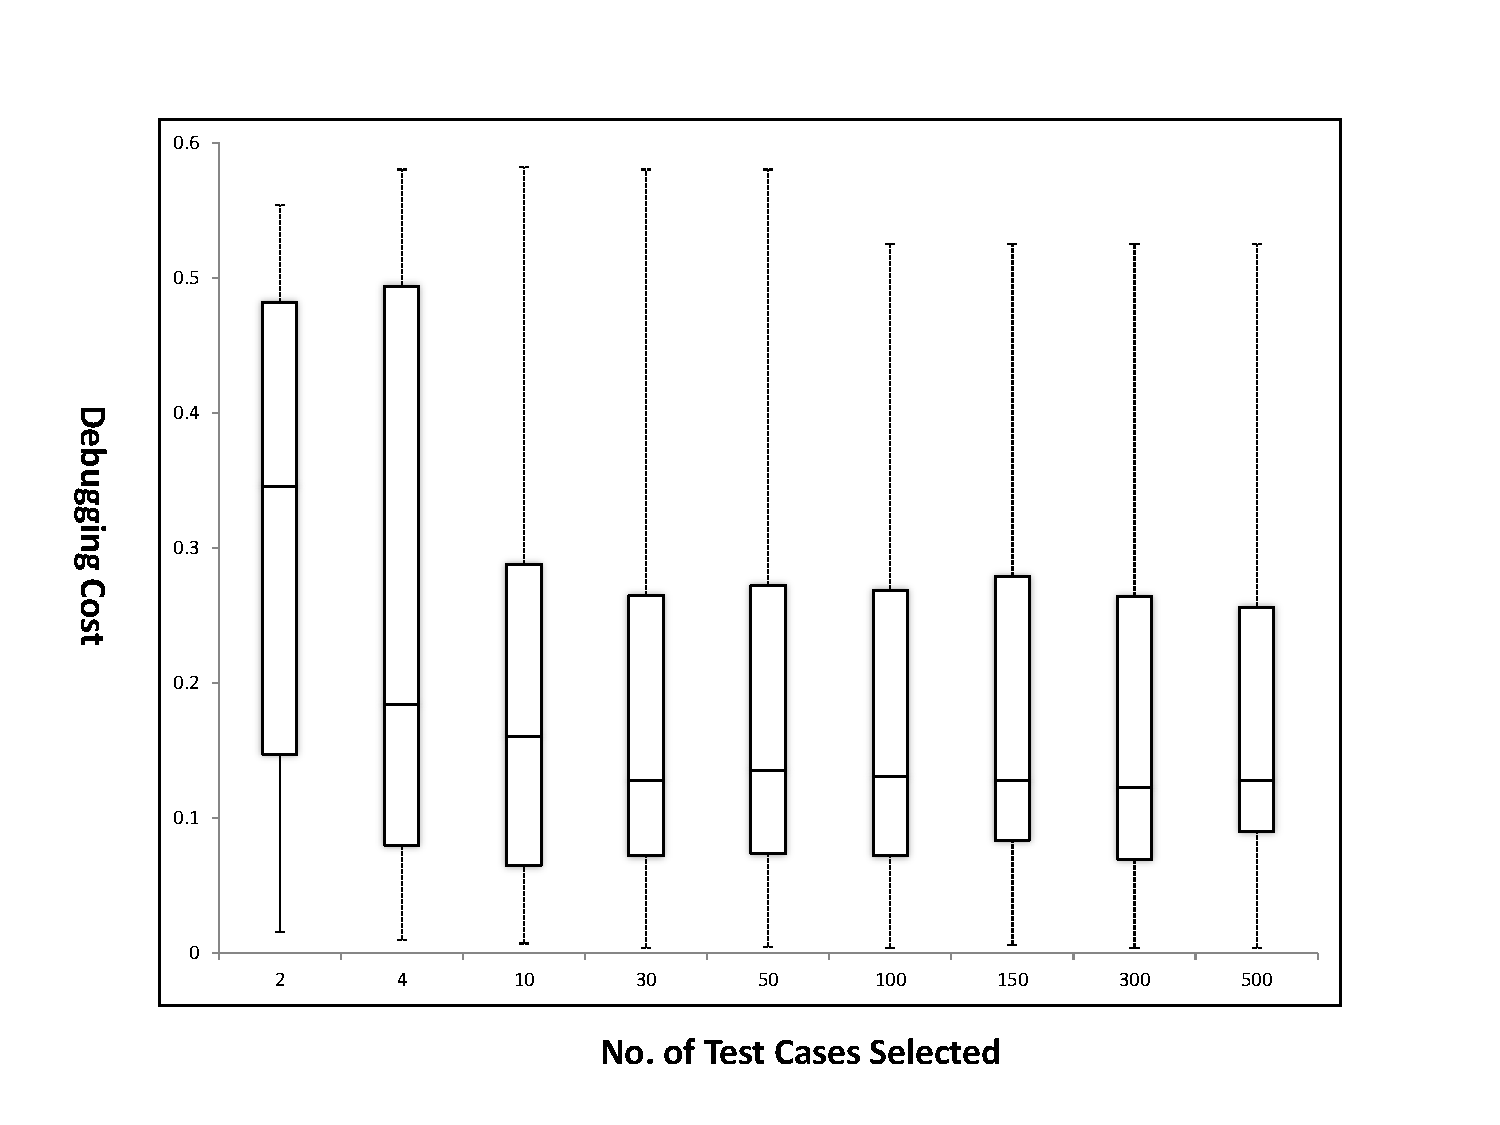
\includegraphics[width=12cm]{mut-sdm.pdf}
    %\vspace{-0.3cm}
    \caption{Average Cost of DMS when Selecting Different Numbers of Test Cases.}\label{fig:costmulti}

\end{figure}

\vspace{0.2cm}
\noindent{\bf Summary.} Table \ref{tab:compare_1}, \ref{tab:compare_2}, and~\ref{tab:compare_2_neg} summarize the comparison between our method and the existing prioritizing techniques, the results show that our method outperforms all of them.

%\vspace{-0.1cm}
\begin{table}[!htbp]
%	\vspace{-8pt}
    \centering
		\caption{Comparison of Prioritization methods.}
		\renewcommand{\arraystretch}{1.5}
		\small
        \begin{tabular}{|c|c|c|c|}
			\hline
			Test Prioritization Method  &  Positive  &  Negative  &   Neutral  \\
			\hline\hline
			\textsc{Dms} vs \textsc{Raptor} & {\bf 34.68\%} &    31.79\% &    33.53\% \\
			\hline
			\textsc{Dms} vs \textsc{Sequoia} & {\bf 46.24\%} &    39.31\% &    14.45\% \\
			\hline
			\textsc{Dms} vs \textsc{Stmt-Addtl} & {\bf 50.29\%} &    28.23\% &    21.39\% \\
			\hline
			\textsc{Dms} vs \textsc{Stmt-Total} & {\bf 71.10\%} &    24.86\% &    4.05\% \\
			\hline
			\textsc{Dms} vs \textsc{Fep-Addtl} & {\bf 51.45\%} &   29.48\% &    19.08\% \\
			\hline
			\textsc{Dms} vs \textsc{Art-Min} & {\bf 71.68\%} &    23.70\% &    4.62\% \\
			\hline
		\end{tabular}
    \label{tab:compare_1}
\end{table}



%\vspace{-0.1cm}
As illustrated in Table \ref{tab:compare_1}, \textsc{Dms} performs better than \textsc{Raptor} on 34.68\% of the faulty versions, worse on 31.79\% of the faulty versions, and shows no improvement on 33.53\% of the faulty versions. The first row of Table~\ref{tab:compare_2} characterizes the degree of positive improvement of \textsc{Dms} over \textsc{Raptor}. As the table indicates, half of the 34.68\% faulty versions with positive improvement values have improvements between 0.03\% and 5.95\%, and the other half have improvements between 5.95\% and 46.75\%. The average positive improvement of \textsc{Dms} over \textsc{Raptor} is 5.95\%.

%
%\vspace{-0.1cm}
\begin{table}[!htbp]
    \centering
		\caption{Distribution of positive improvements.}
		\renewcommand{\arraystretch}{1.5}
		\small
        \begin{tabular}{|c|c|c|c|c|}
			\hline
			Test Prioritization Method  &        Max &       Mean &     Median &        Min \\
			\hline\hline
			\textsc{Dms} vs \textsc{Raptor} & {  46.75\%} &     5.95\% &     1.05\% &     0.03\% \\
			\hline
			\textsc{Dms} vs \textsc{Sequoia} & {  51.75\%} &   18.31\% &     14.31\% &     0.56\% \\
			\hline
			\textsc{Dms} vs \textsc{Stmt-Addtl} & {   54.24\%} &    10.67\% &     4.50\% &     0.04\% \\
			\hline
			\textsc{Dms} vs \textsc{Stmt-Total} & {  56.31\%} &    19.25\% &    25.42\% &     0.19\% \\
			\hline
			\textsc{Dms} vs \textsc{Fep-Addtl} & {  99.05\%} &    17.94\% &     9.04\% &     0.02\% \\
			\hline
			\textsc{Dms} vs \textsc{Art-Min} & {  99.13\%} &     42.96\% &     36.83\% &     0.14\% \\
			\hline
		\end{tabular}
    \label{tab:compare_2}
\end{table}


\begin{table}[!htbp]
    \centering
		\caption{Distribution of negative improvements.}
		\renewcommand{\arraystretch}{1.5}
		\small
        \begin{tabular}{|c|c|c|c|c|}
			\hline
			Test Prioritization Method  &        Max &       Mean &     Median &        Min \\
			\hline\hline
			\textsc{Dms} vs \textsc{Raptor} & {  53.30\%} &     8.54\% &     2.94\% &     0.23\% \\
			\hline
			\textsc{Dms} vs \textsc{Sequoia} & {  52.00\%} &   8.49\% &     4.37\% &     0.19\% \\
			\hline
			\textsc{Dms} vs \textsc{Stmt-Addtl} & {  53.86\%} &    10.88\% &     4.87\% &     0.14\% \\
			\hline
			\textsc{Dms} vs \textsc{Stmt-Total} & { 51.38\%} &   10.56\% &   7.10\% &     0.13\% \\
			\hline
			\textsc{Dms} vs \textsc{Fep-Addtl} & {  47.13\%} &    10.72\% &     5.89\% &     0.04\% \\
			\hline
			\textsc{Dms} vs \textsc{Art-Min} & {  46.21\%} &     3.33\% &     2.01\% &     0.16\% \\
			\hline
		\end{tabular}
    \label{tab:compare_2_neg}
\end{table}

We conduct paired Wilcoxon signed-rank test to confirm the difference in performance between \textsc{Dms} and six existing prioritization techniques. The statistical test result rejects the null hypothesis and suggests that \textsc{Dms} is statistically significantly better than the existing best approach on the multi-fault subject programs at 95\% confidence interval.

\vspace{0.2cm}\noindent{\bf Detailed Comparison.}
Table \ref{fig:costmulti} shows that \textsc{Raptor}, \textsc{Fep-Addtl} and \textsc{Art-Min} achieve 101\% base line effectiveness with less than 500 test cases on subject programs. We only show the comparison between \textsc{Dms} and these methods in detail. Figure~\ref{fig:our_vs_fep}, \ref{fig:our_vs_artmin}, and~\ref{fig:our_vs_ag_unix} show the comparison between different prioritization techniques based on fault localization cost.

\vspace{0.2cm}\noindent{\bf D{\scriptsize MS} vs F{\scriptsize EP}-A{\scriptsize DDTL}.}
Figure \ref{fig:our_vs_fep} presents the comparison between \textsc{Dms} and \textsc{Fep-Addtl} over all faulty versions. The comparison shows that \textsc{Dms} is better than \textsc{Fep-Addtl}. Out of 140 versions that show differences in Costs, our prioritization method performs better than \textsc{Fep-Addtl} on 89 versions but performs worse than the \textsc{Fep-Addtl} on 51 versions. The positive improvement ranges from 0.02\% to 99.05\%, with an average of 17.94\%.

%Previous studies~\cite{RUCH01,SEAGMGR01} show that \textsc{Fep-Addtl} is the most promising prioritizing method for fault detection.
%However \textsc{Fep-Addtl} is not suitable for diagnostic prioritization,
%since it is initially proposed for regression testing, which assumes that
%tester have already get test oracles for each test case. But measuring
%{\em FEP} requires test oracles for all test cases which are absent in our problem.
%As a result, without test oracles {\em FEP} cannot evaluate the fault
%detection rate of each test case on program mutants.
%To circumvent this problem, Alberto \etal~\cite{Gonzalez-SanchezPAGG11} approximated {\em FEP}
%Without test oracles, \textsc{Fep} can be estimated by $1 - ${\em False Negative Rate} (\textsc{Fnr})~\cite{Gonzalez-SanchezPAGG11}
%\footnote{\textsc{Fnr} is the program passing rate when program element is the real fault and executed in test case. Usually when
%\textsc{Fnr} is high, the fault is difficult to be detected by Spectrum-based
%fault localization techniques.} which is also used in our study.

\begin{figure}[!htbp]
    \centering
    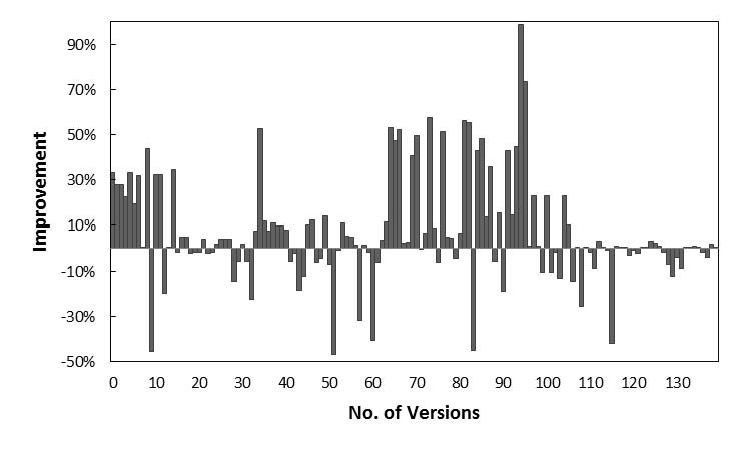
\includegraphics[width=12cm]{mut-dms-feq.pdf}
%    \vspace{-0.3cm}
\caption{Improvement of D{\scriptsize MS} over F{\scriptsize EP}-A{\scriptsize DDTL}.}
    \label{fig:our_vs_fep}
\end{figure}
%\vspace{0.2cm}



\begin{figure}[!htbp]
    \centering
    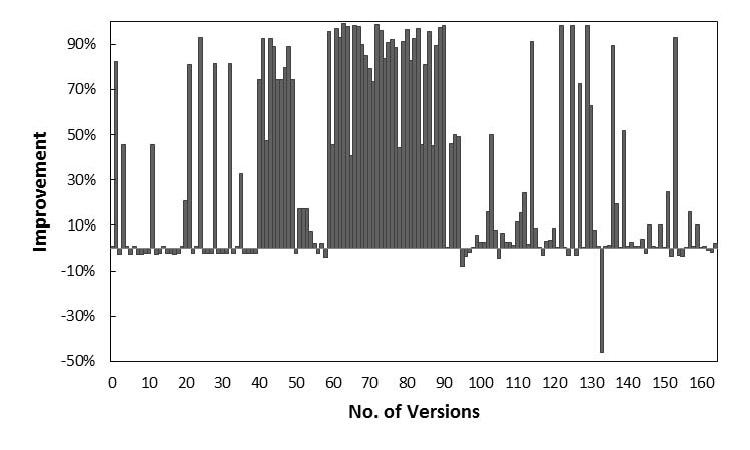
\includegraphics[width=12cm]{mut-dms-art.pdf}
%    \vspace{-0.3cm}
    \caption{Improvement of D{\scriptsize MS} over A{\scriptsize rt}-M{\scriptsize IN}.}
    \label{fig:our_vs_artmin}
\end{figure}

%\vspace{0.2cm}
\vspace{0.2cm}\noindent{\bf D{\scriptsize MS} vs A{\scriptsize rt}-M{\scriptsize IN}.}
We compare the effectiveness of \textsc{Dms} to the best variant of {\em Adaptive Random Test Prioritization}(\textsc{Art}), namely \textsc{Art-Min}~\citep{JiangZCT09, Gonzalez-SanchezPAGG11, Alberto2011}. Figure \ref{fig:our_vs_artmin} shows the results of the study in which \textsc{Art-Min} is used as the baseline method. The comparison shows that \textsc{Dms} is better than \textsc{Art-Min}. Out of 165 versions that show differences in Costs, our prioritization method performs better than \textsc{Art-Min} on 124 versions but performs worse than the \textsc{Art-Min} on 41 versions.

%The positive improvement ranges from 0.03\% to 53.81\%, with an average of 7.70\%.

\vspace{0.2cm}\noindent{\bf D{\scriptsize MS} vs R{\scriptsize APTOR}.}
Figure \ref{fig:our_vs_ag_unix} shows the comparison between \textsc{Dms} and \textsc{Raptor}. The comparison shows that \textsc{Dms} is better than \textsc{Raptor}.  Out of 115 versions that show differences in Costs, our prioritization method performs better than \textsc{Raptor} on 60 versions but performs worse than the \textsc{Raptor} on 55 versions.

%\textsc{Dms} outperforms \textsc{Raptor} on 20 versions by at least 1\% cost, and only 5 versions worse than \textsc{Raptor} over 1\% cost.

\begin{figure}[!htbp]
    \centering
    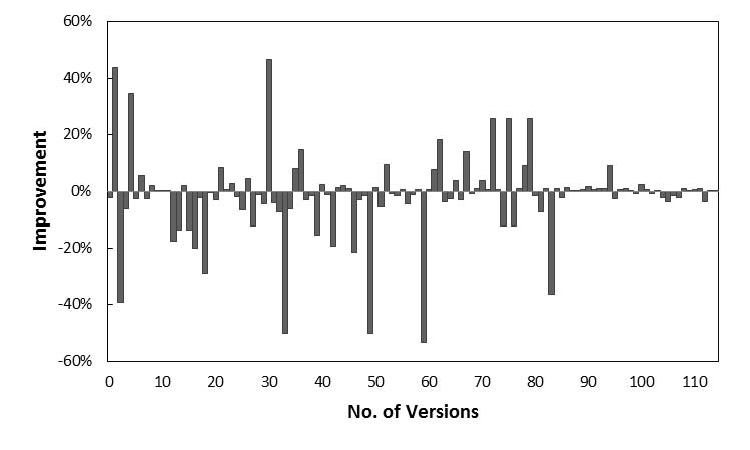
\includegraphics[width=12cm]{mut-dms-raptor.pdf}
%    \vspace{-0.3cm}
\caption{Improvement of D{\scriptsize MS} over R{\scriptsize APTOR}.}
    \label{fig:our_vs_ag_unix}
\end{figure}

%on U{\scriptsize NIX} programs

%There is also improvement on Siemens programs: 32.2\% versions show differences and the average debugging cost improvement is 1.3\%, which is not so significant as comparison on \textsc{Unix} programs.
%This is probably due to the small software size. On Siemens programs the existing best approach
%can reach 101\% of the base line effectiveness by only selecting less than 20 test cases on average (see Table \ref{tab:label_effort}).
%By selecting such few test cases, \textsc{Raptor} already obtains the maximal ambiguity group reduction due to very limited different
%coverage profiles. For example, all test cases of \texttt{tcas} only have less than 15 ambiguity groups in all faulty versions. In this case,
%the speedup by our method is trivial. In real scenario, programs to be diagnosed would be more similar to \textsc{Unix} programs.
